\chapter{annexe}

\section{Lexique}

\textbf{Flux}
Un flux permet l'envoi et la reception de données. Ils traitent les données de manière séquentielle ou asynchrones.



\textbf{Swift}


\begin{figure} %on ouvre l'environnement figure
\centering
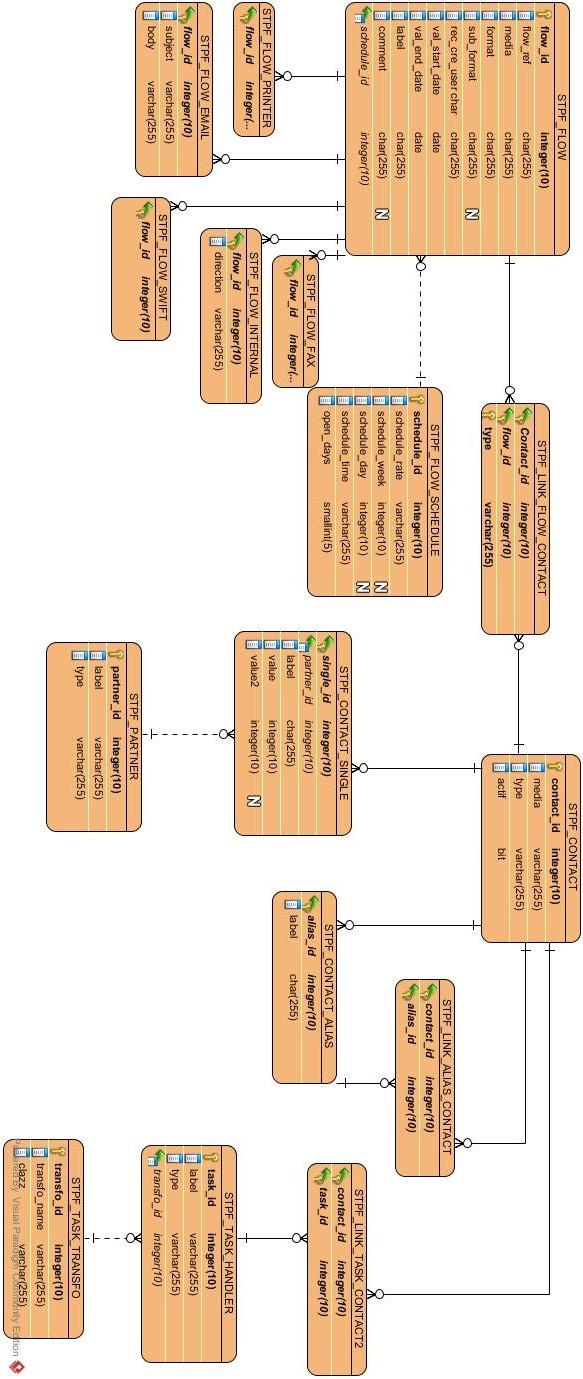
\includegraphics[scale=0.6]{Images/FlowDetailsExistant.jpg}
\caption{Diagramme entité relation de la modélisation existante} %la légende
\end{figure} %on ferme l'environnement figure

\newpage
\begin{figure} %on ouvre l'environnement figure
\centering
\includegraphics[width=14cm, height=23cm]{Images/Gantt.png}
\caption{Diagramme de Gantt} %la légende
\end{figure} %on ferme l'environnement figure